
\documentclass[a4paper]{article}

%% Language and font encodings
\usepackage[english]{babel}
\usepackage[utf8x]{inputenc}
\usepackage[T1]{fontenc}

%\bibliographystyle{apalike} %% Sets page size and margins
\usepackage[round]{natbib}
\bibliographystyle{plainnat}
%\usepackage[a4paper,top=3cm,bottom=2cm,left=3cm,right=3cm,marginparwidth=1.75cm]{geometry}

%% Useful packages
\usepackage{amsmath}
\usepackage{graphicx}
\usepackage[colorinlistoftodos]{todonotes}
\usepackage[colorlinks=true, allcolors=blue]{hyperref}
\usepackage{subfigure} 
\usepackage{float}

\graphicspath{{../plots/}}

\usepackage{listings,xcolor}

\title{Análisis de series de tiempo para el reconocimiento de ciclos económicos.}
\author{Pablo Santoro, Diego Kozlowski}

\begin{document}

\maketitle

\begin{abstract}
	
La regularidad de ciclos económicos de diversa duración en economías de mercado es un tópico objeto de numerosos trabajos y debates a lo largo de la historia del pensamiento económico para comprender las causas subyacentes a los períodos de expansión y contracción propio del sistema de reproducción capitalista. En el siguiente trabajo se busca evidencia empírica acerca de las de estos ciclos económicos en diversas frecuencias en distintas mediciones de largo plazo hechas a variables macroeconómicas de la economía de los EE.UU.
\end{abstract}

\section{Análisis de ciclos de baja frecuencia en series de tiempo de variables macroeconómicas}
\subsection{Tasa de interés de largo plazo}

En el siguiente apartado se analizan los ciclos que se pueden detectar en la serie de tasas de interés de largo plazo de los bonos del Tesoro de los EE.UU.
\todo{revisar que sean los bonos del Tesoro de los EE.UU.}
En la figura \ref{fig:ir_orig} se puede observar la serie de tasas de interés de largo plazo por año. En la misma se puede observar una diferencia significativa en el nivel de tasas de la segunda mitad del siglo XX respecto de los años anteriores, sobre todo posteriores a 1970. Esto corresponde a niveles altos de inflación en los EE.UU. en este periodo y la siguiente paulatina baja de la inflación llegando al siglo XXI.

\begin{figure}[H]
	\centering
	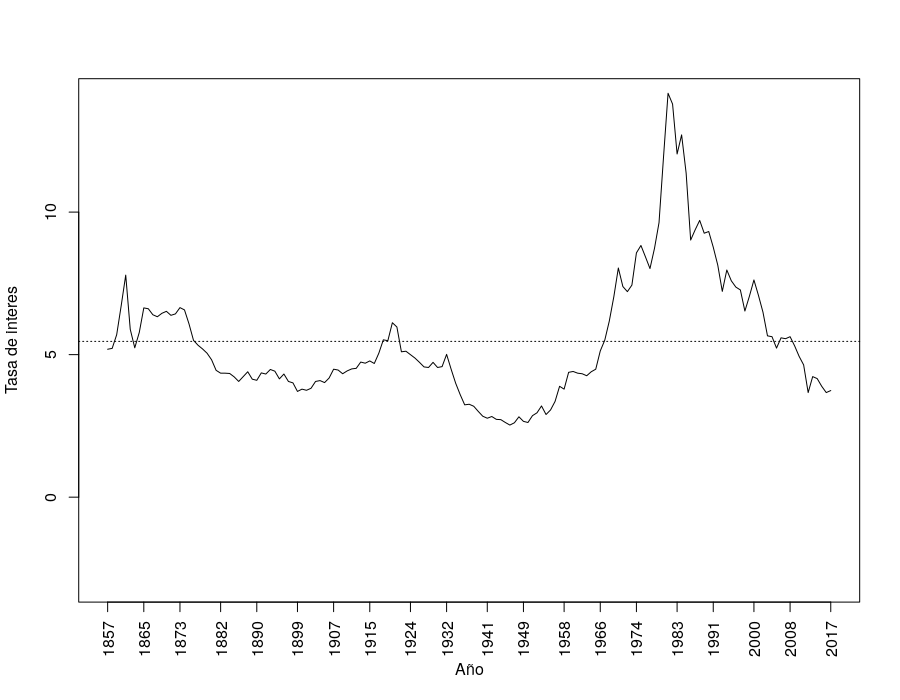
\includegraphics[width=0.75\linewidth]{ir_orig.png}
	
	\caption{Tasa de interés de largo plazo de los EE.UU.}
	\label{fig:ir_orig}
\end{figure}

A continuación (Figura \ref{fig:ir_diff_acf}) se muestran el gráficos de diferencias (cambios absolutos, en puntos porcentuales, de la tasa de interés de largo plazo, por año) y la autocorrelación de las diferencias. Se observa que hay una leve correlación con el periodo siguiente al lag 0, pero en general la autocorrelación es muy similar a un random walk.

\begin{figure}[H]
	\centering
	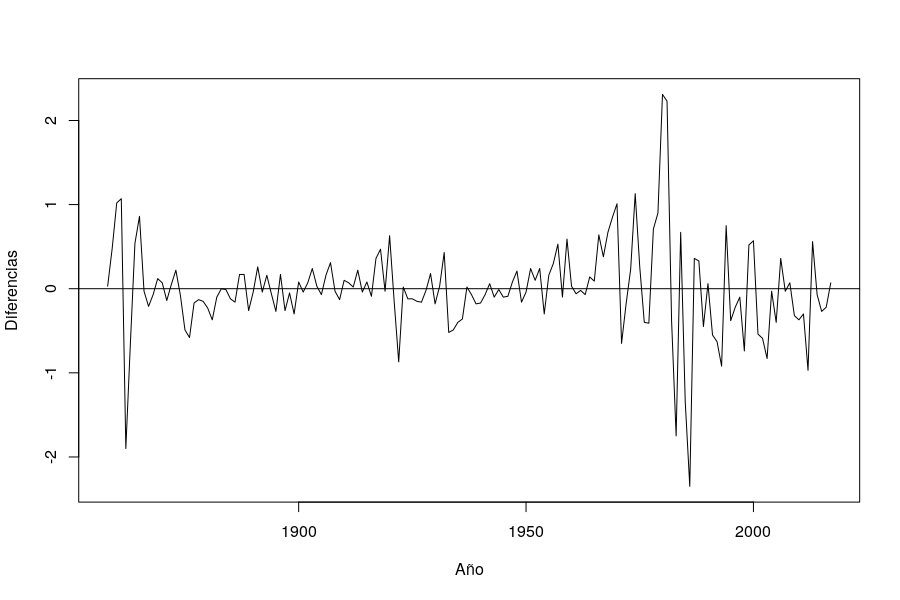
\includegraphics[width=0.75\linewidth]{ir_diff.png}
	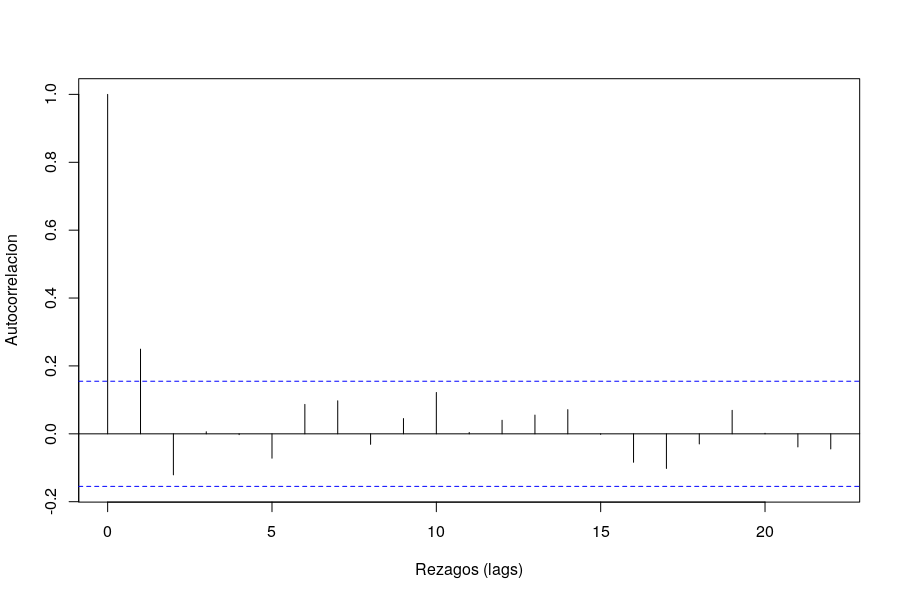
\includegraphics[width=0.75\linewidth]{ir_diff_acf.png}
	\caption{Diferencias (arriba) y autocorrelación de las diferencias (abajo) de las tasas de interes.} 	
	\label{fig:ir_diff_acf}
\end{figure}

Si bien no se observan tendencias de largo plazo en las diferencias y estas sirven habitualmente para centrar las series, la diferenciación sólo captura las frecuencias más altas, dejando de lado las de largo plazo, por lo que con este análisis sólo se pueden investigar ciclos de corta duración. Para poder investigar ciclos de mayor duración se investiga la transformada de Fourier de la serie, que permite observar las frecuencias y amplitudes que componen la serie. En la figura \ref{fig:ir_fft} puede observarse el espectro de frecuencias de la serie de tasas de interés centrada en su media.

\begin{figure}[H]
	\centering
	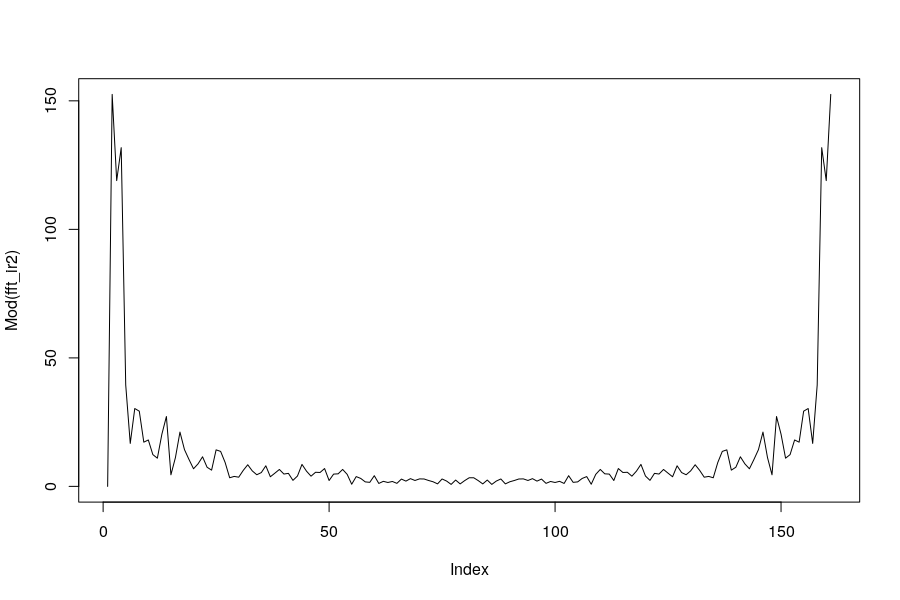
\includegraphics[width=0.8\linewidth]{ir_fft.png}
	\caption{Transformada de Fourier de la tasa de interés} 	
	\label{fig:ir_fft}
\end{figure}

Se observa que hay frecuencias bajas con gran amplitud. Si descomponemos la serie por las frecuencias más bajas, se puede observar la serie en rojo de la figura \ref{fig:ir_orig_resid} que resulta de la descomposición de la serie original por las frecuencias más bajas. Puede observarse que la serie aún presenta autocorrelación (en detalle la autocorrelación de la figura \ref{fig:ir_resid_acf})

\begin{figure}[H]
	\centering
	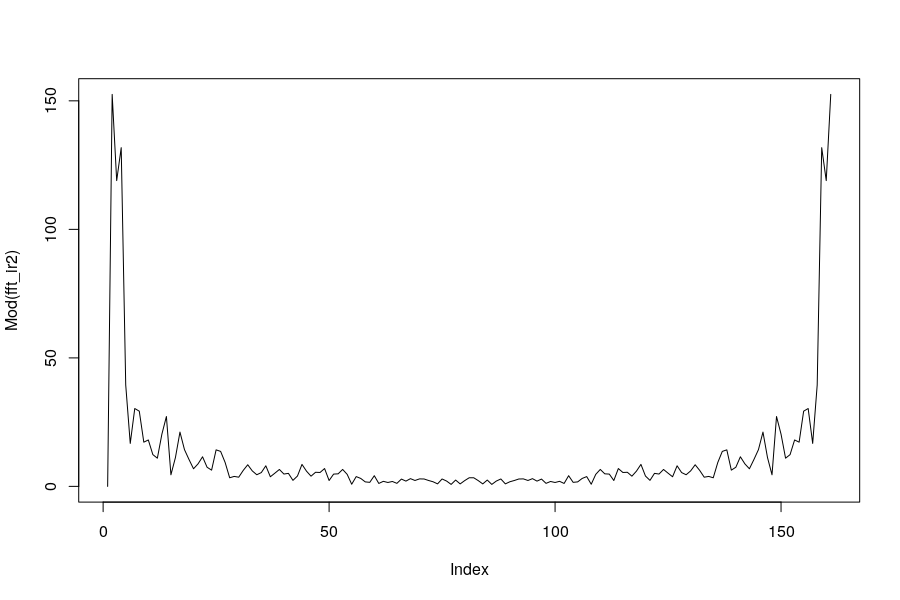
\includegraphics[width=0.8\linewidth]{ir_fft.png}
	\caption{Serie original y residuos (en rojo) de descomponer por las frecuencias más bajas} 	
	\label{fig:ir_orig_resid}
\end{figure}

\begin{figure}[H]
	\centering
	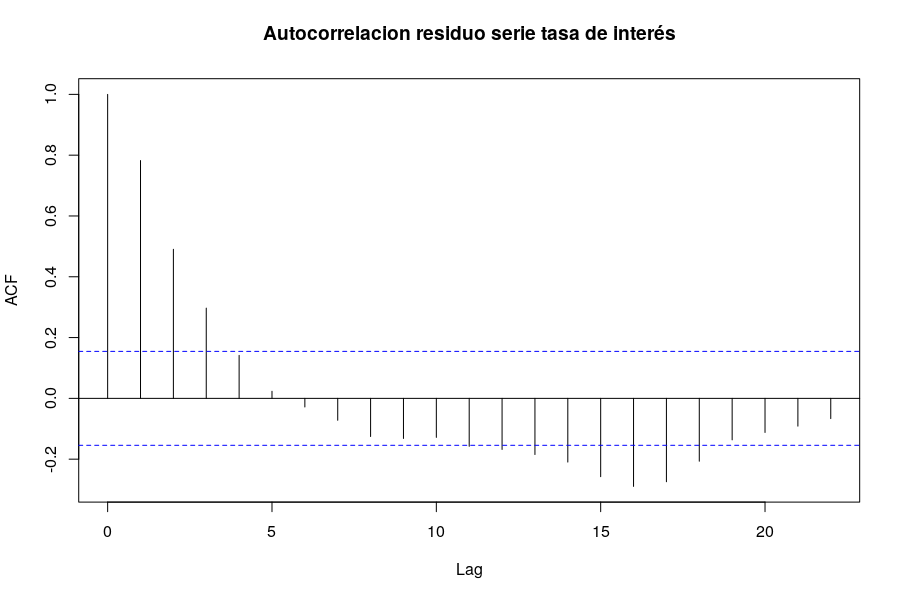
\includegraphics[width=0.8\linewidth]{ir_resid_acf.png}
	\caption{Autocorrelación de la parte no explicada por la descomposición de las frecuencias más bajas} 	
	\label{fig:ir_resid_acf}
\end{figure}

\subsection{Índice de precios al consumidor}
La serie de nivel de precios al consumidor(\textit{"Consumer Price Index"}, Índice de precios al consumidor, \textit{CPI} por sus siglas en inglés, \textit{IPC} en español) de los EE.UU. está expresada en base 100, con base en el promedio anual de 1982-1984. La serie de tiempo original se puede observar en la figura \ref{fig:cpi_orig}, donde se observa el fenómeno exponencial de la inflación a través de los años. Asimismo, se puede observar una diferencia entre los siglos XIX y XX, especialmente tras el rompimiento con el sistema de patrón oro de 1971 durante la administración Nixon y los años previos al abandono de este sistema de respaldo de papel moneda. Este hecho de diferencias seculares en el nivel de precios puede observarse con mayor detalle en la figura \ref{fig:cpi_log10_tend} donde se observa el logaritmo en base diez de los datos originales con tendencias lineales calculadas para los años previos y posteriores a 1900, apreciandose el cambio de tendencia del crecimiento del nivel de precios. En este último gráfico se han marcado también con líneas punteadas rojas acontecimientos notables de la historia de los EE.UU. y mundiales para tomar como referencia en los cambios de estas variables macroeconómicas.

\begin{figure}[H]
	\centering
	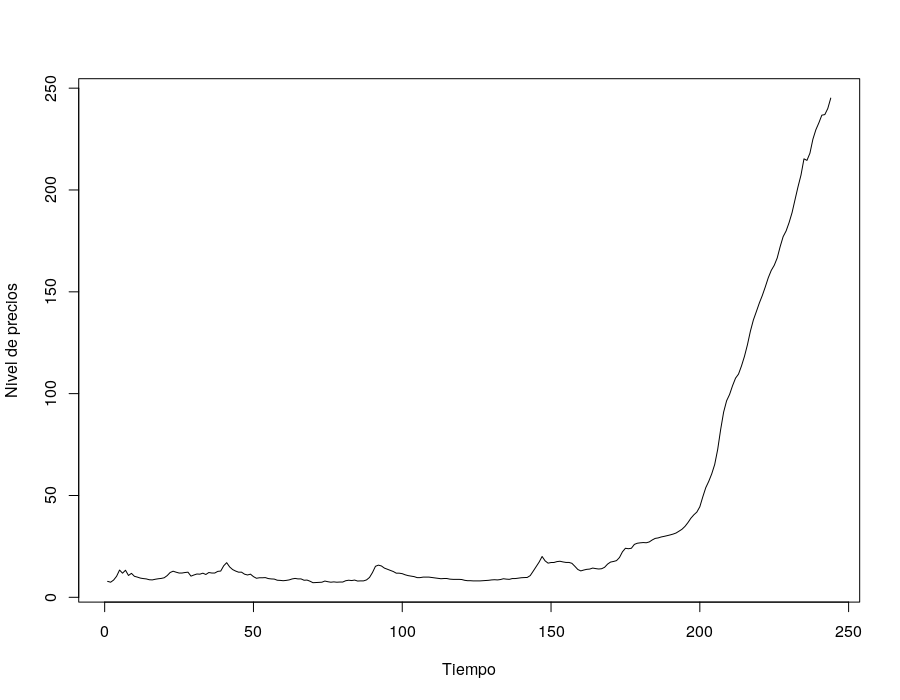
\includegraphics[width=0.8\linewidth]{cpi_orig.png}
	\caption{Índice de precios al consumidor en los EE.UU., base: promedio anual de 1982-1984} 	
	\label{fig:cpi_orig}
\end{figure}

\begin{figure}[H]
	\centering
	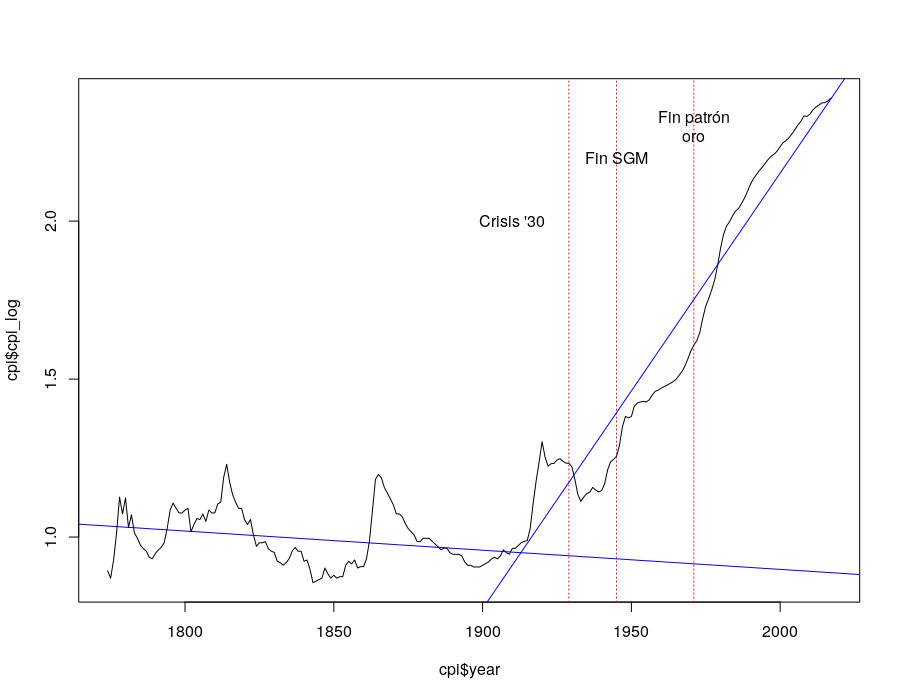
\includegraphics[width=0.8\linewidth]{cpi_log10_tend.png}
	\caption{Log 10 y tendencias ajustadas antes y después del año 1900} 	
	\label{fig:cpi_log10_tend}
\end{figure}

Se elige centrar la serie de precios por las tendencias lineales para poder evitar que se distorsione el ciclo usando técnicas que ajusten mejor a datos no lineales, debido a que se analizarán los residuos de estas series con transformaciones de Fourier en busca de poder explicarlos y de buscar la existencia de ciclos alrededor de estas tendencias. Se pueden observar las tendencias centradas y la alternancia alrededor de cero en la figura \ref{fig:cpi_log10_cntr}.

\begin{figure}[H]
	\centering
    \subfigure{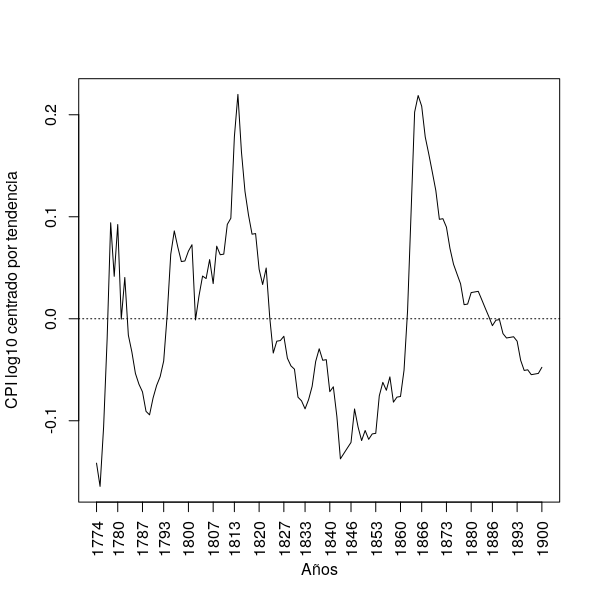
\includegraphics[width=0.49\linewidth]{cpi_log10_cntr_pre.png}}
	\subfigure{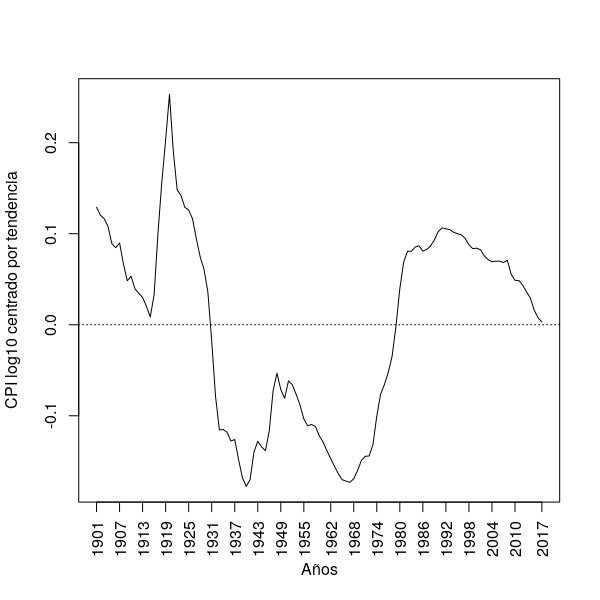
\includegraphics[width=0.49\linewidth]{cpi_log10_cntr_post.png}}
	\caption{IPC log10 centrado por tendencia lineal antes (izquierda) y después (derecha) de 1900} 	
	\label{fig:cpi_log10_cntr}
\end{figure}

Pasamos ahora al análisis de los residuos: la serie centrada por las tendencias. Realizamos las transformadas de Fourier sobre estas nuevas series. El resultado puede observarse en la figura \ref{fig:cpi_log10_cntr_fft}, en la que puede verse que las frecuencias más bajas son las que cuentan con mayor amplitud.

\begin{figure}[H]
	\centering
    \subfigure{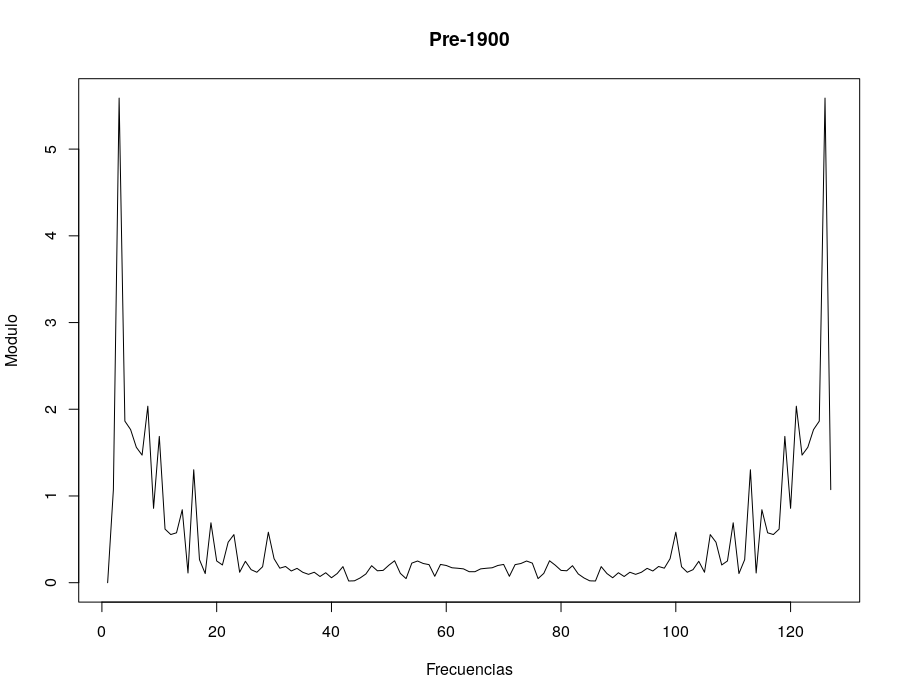
\includegraphics[width=0.49\linewidth]{cpi_fft_pre1900.png}	}
	\subfigure{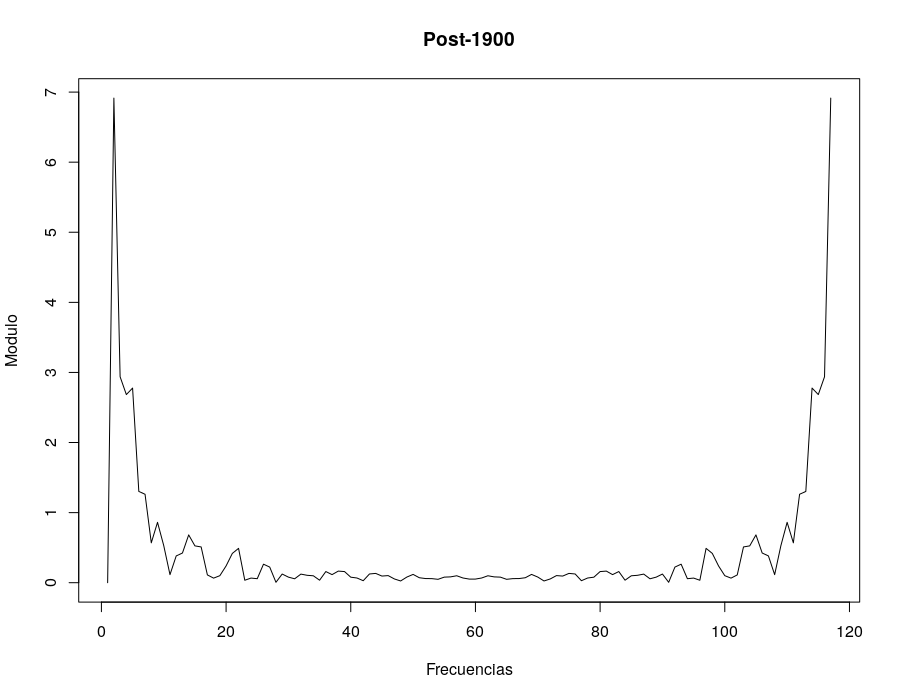
\includegraphics[width=0.49\linewidth]{cpi_fft_post1900.png}}
	\caption{IPC log10 centrado por tendencia lineal antes (izquierda) y después (derecha) de 1900} 	
	\label{fig:cpi_log10_cntr_fft}
\end{figure}

Ahora podemos tomar las frecuencias más bajas y descomponer la serie centrada por ellas, analizar el ajuste de estas nuevas series y visualizar la serie resultante de esta descomposición. En la figura \ref{fig:cpi_cntr_antifft} se pueden observar las primeras 9 componentes de más baja frecuencia de la transformada de Fourier y, en azul, el residuo de restar los valores de la transformación de la serie de tiempo. En la figura \ref{fig:cpi_cntr_acf} puede observarse también que aún puede continuar explicándose los residuos en azul debido a que hay rezagos que tienen correlación entre sí. Esto demuestra que, si bien existen ciclos de bajas frecuencias pueden descomponerse series de más altas frecuencias que corresponderían a ciclos de medio y corto plazo.

\begin{figure}[H]
	\centering
    \subfigure{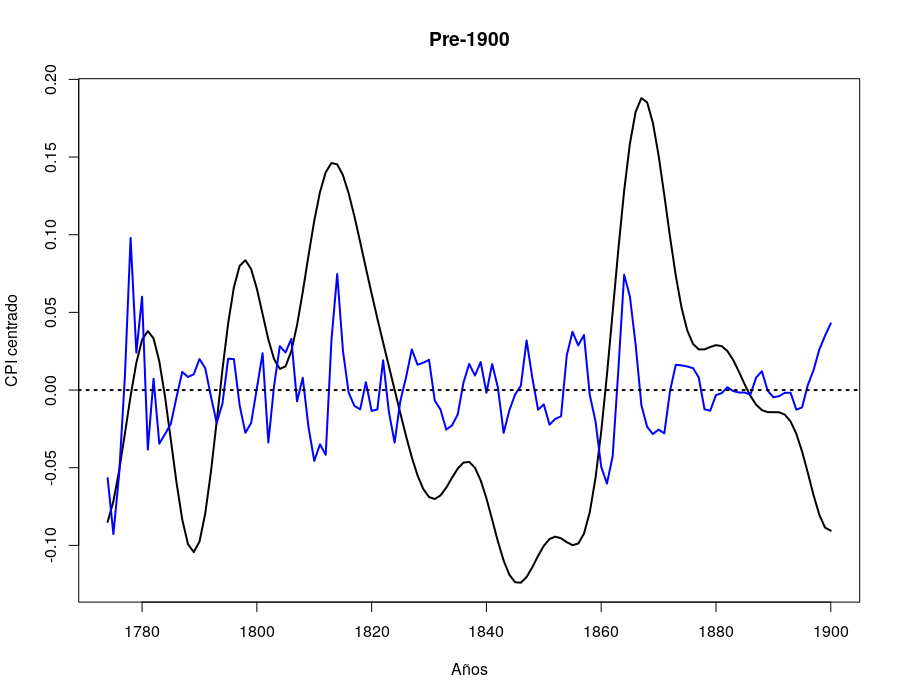
\includegraphics[width=0.49\linewidth]{cpi_antifft_pre1900.png}}
	\subfigure{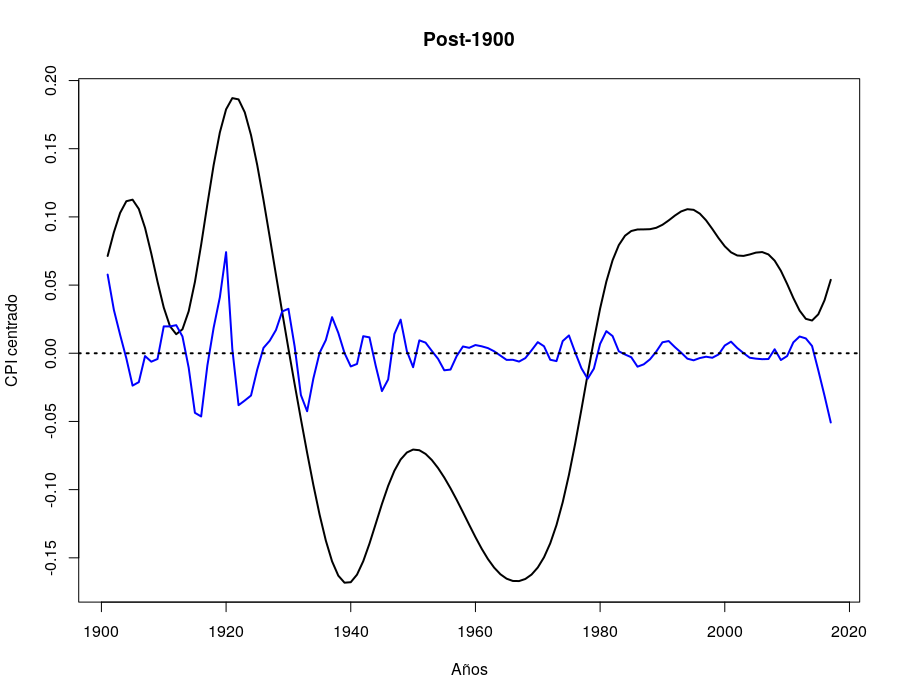
\includegraphics[width=0.49\linewidth]{cpi_antifft_post1900.png}}
	\caption{Residuos (en azul) luego de quitar las bajas frecuencias} 	
	\label{fig:cpi_cntr_antifft}
\end{figure}

\begin{figure}[H]
	\centering
    \subfigure{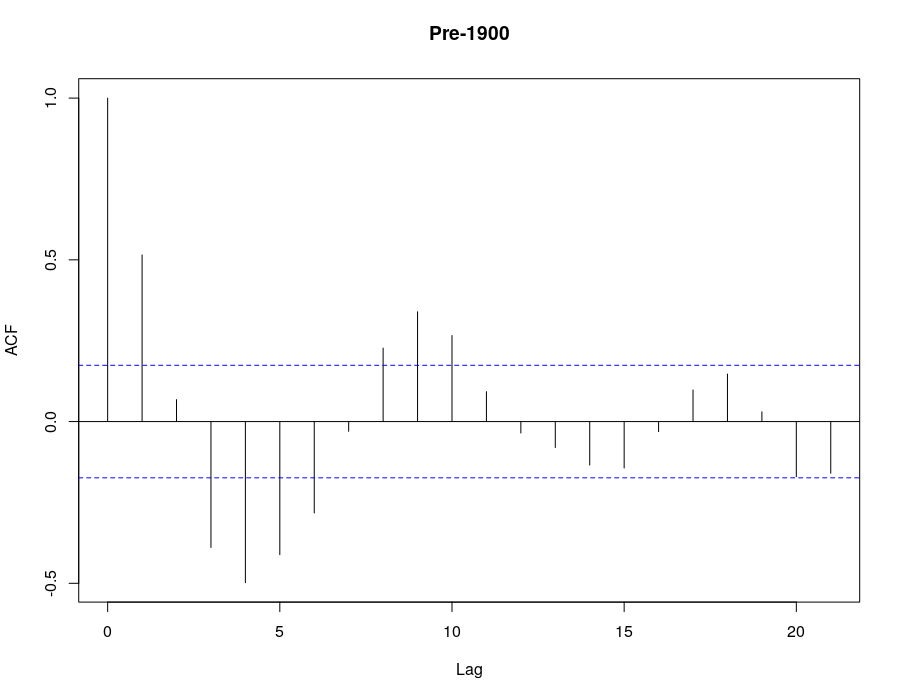
\includegraphics[width=0.49\linewidth]{cpi_acf_pre1900.png}}
	\subfigure{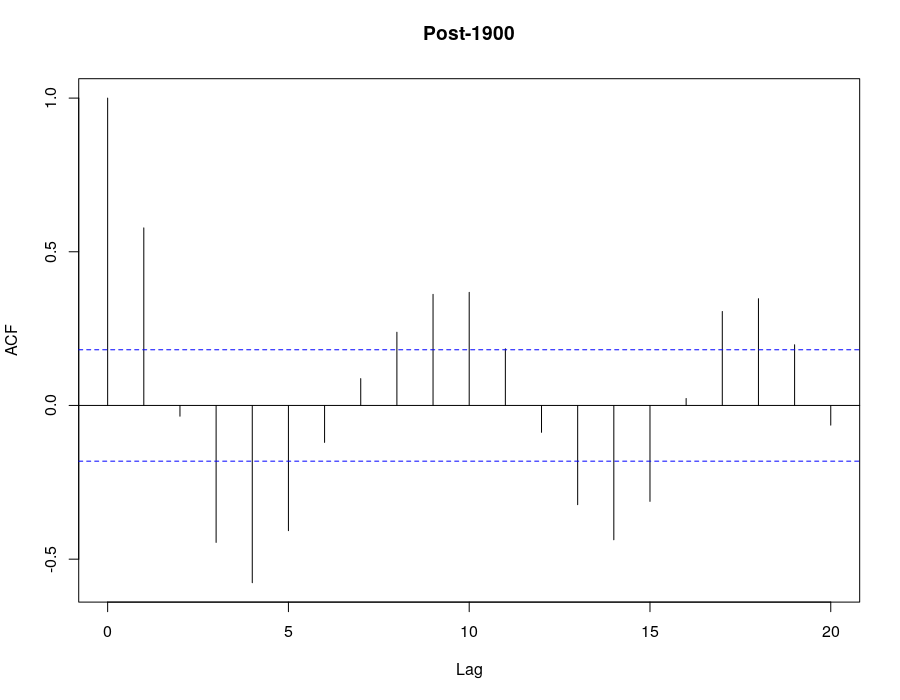
\includegraphics[width=0.49\linewidth]{cpi_acf_post1900.png}}
	\caption{Autocorrelación de los residuos}
	\label{fig:cpi_cntr_acf}
\end{figure}

\subsection{PBI real}
Estados Unidos se ha convertido en la economía más poderosa del mundo con el transcurrir de los años desde su independencia por diversos factores. Más allá de las crisis y eventos significativos como pueden ser las guerras mundiales, la Guerra Fría, el abandono del patrón oro y un sinfín de políticas económicas de diverso tenor, uno de los efectos más notables es la forma en que sostiene un crecimiento de muy largo plazo casi constante a lo largo de su historia reciente. Esto se puede visualizar en la figura \ref{fig:PBI_orig} en donde, a la izquierda se puede visualizar el PBI real de los EE.UU. y a la derecha, el logaritmo en base 10 de la serie de la izquierda en donde además se ajustó una linea mediante mínimos cuadrados (regresión lineal) ilustrando la tendencia. El ajuste es muy bueno, con un R cuadrado de 99.54\%, lo que demuestra que casi se mantiene constante la tasa de crecimiento a lo largo de todo el periodo considerado en la serie.

\begin{figure}[H]
	\centering
    \subfigure{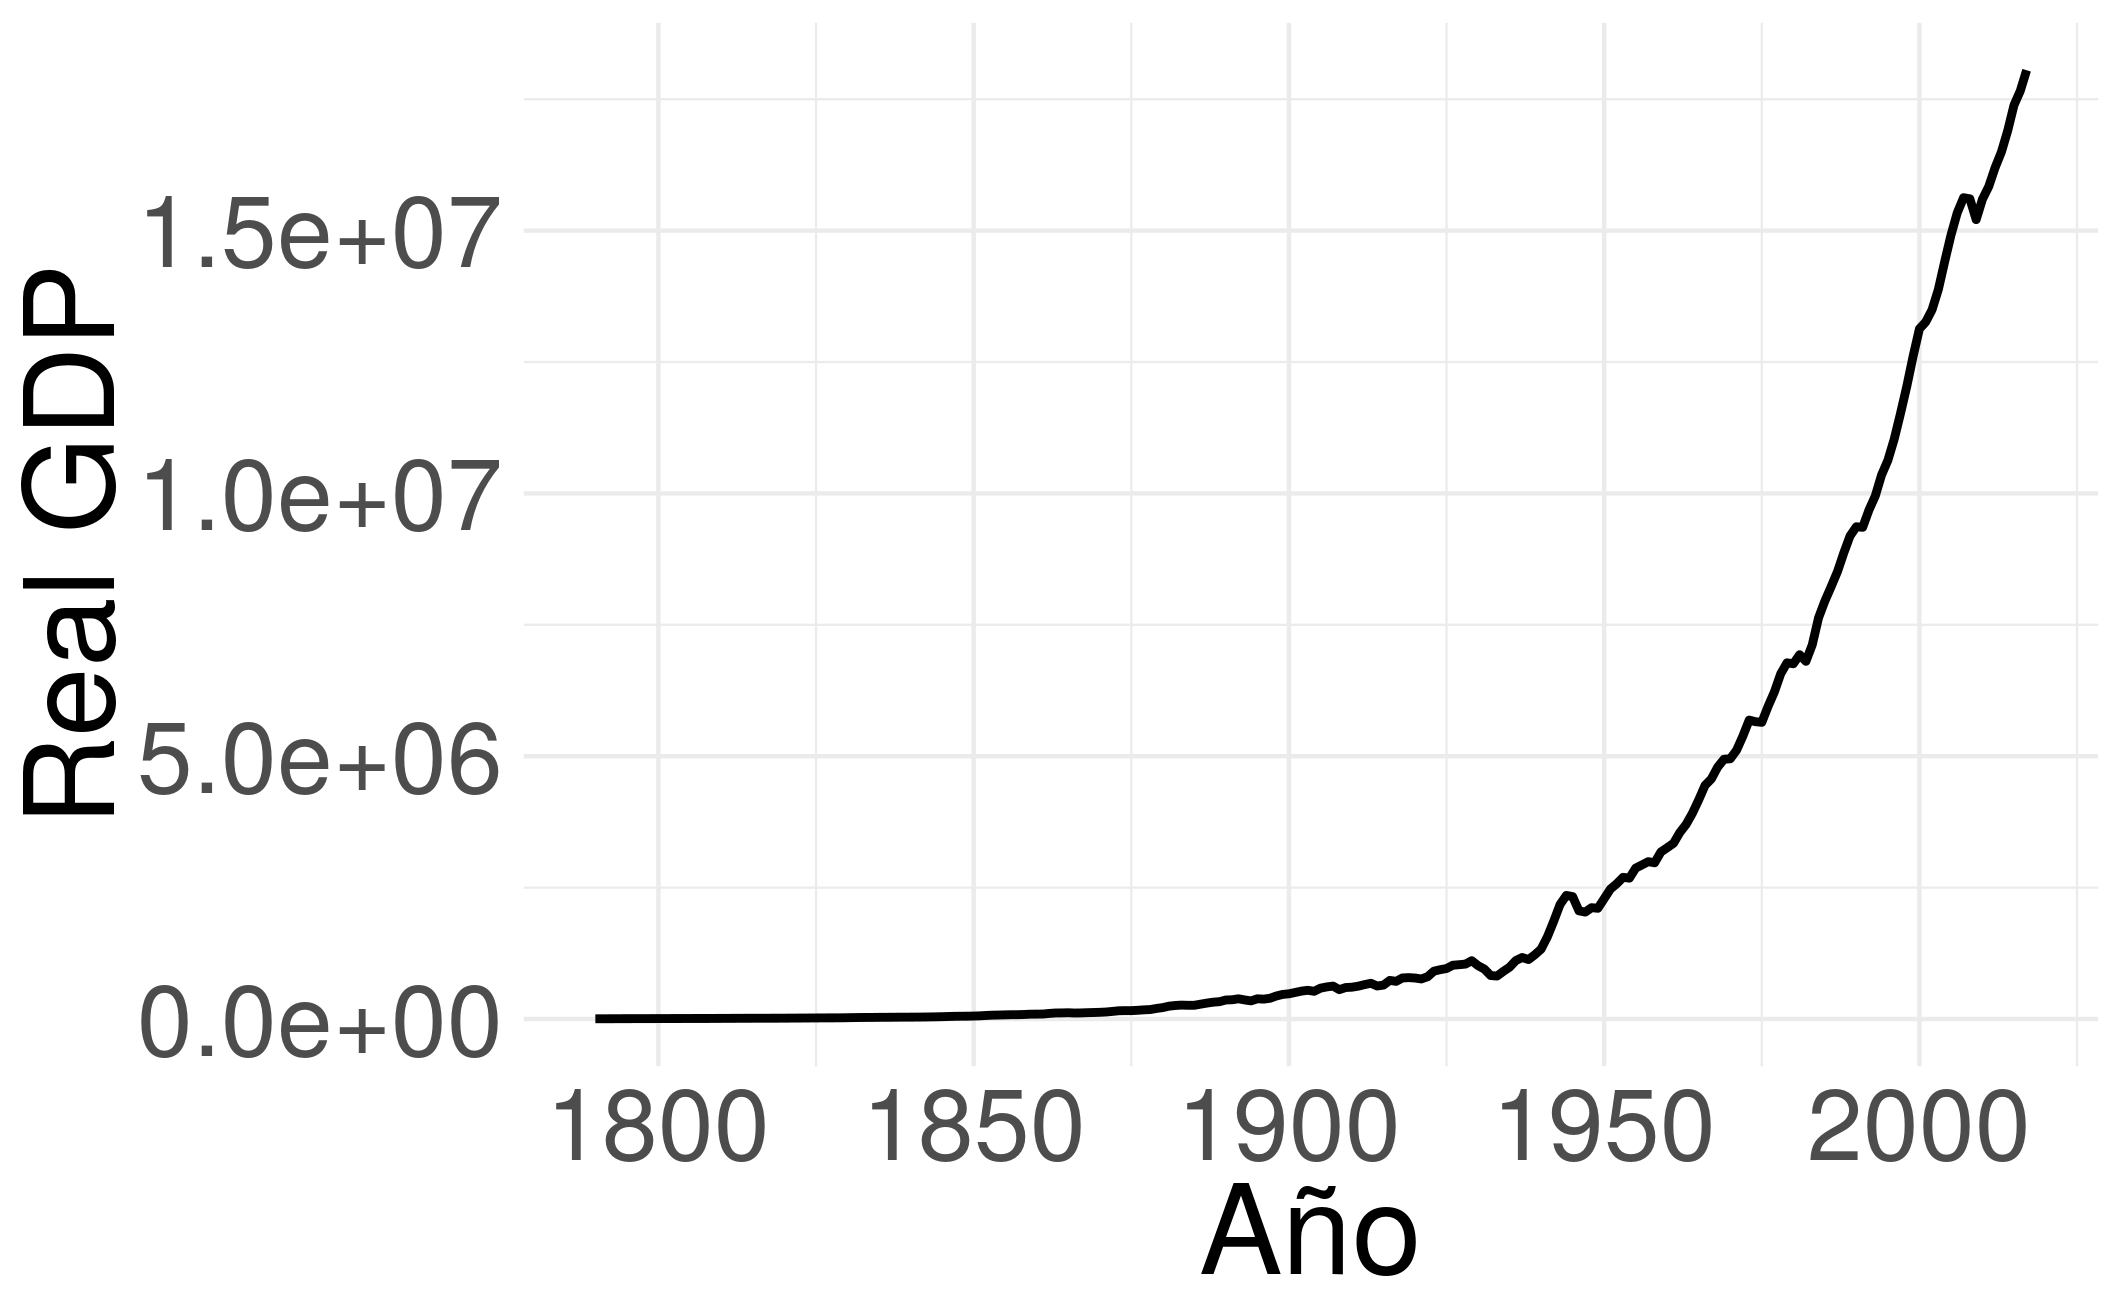
\includegraphics[width=0.49\linewidth]{PBI.png}	}
	\subfigure{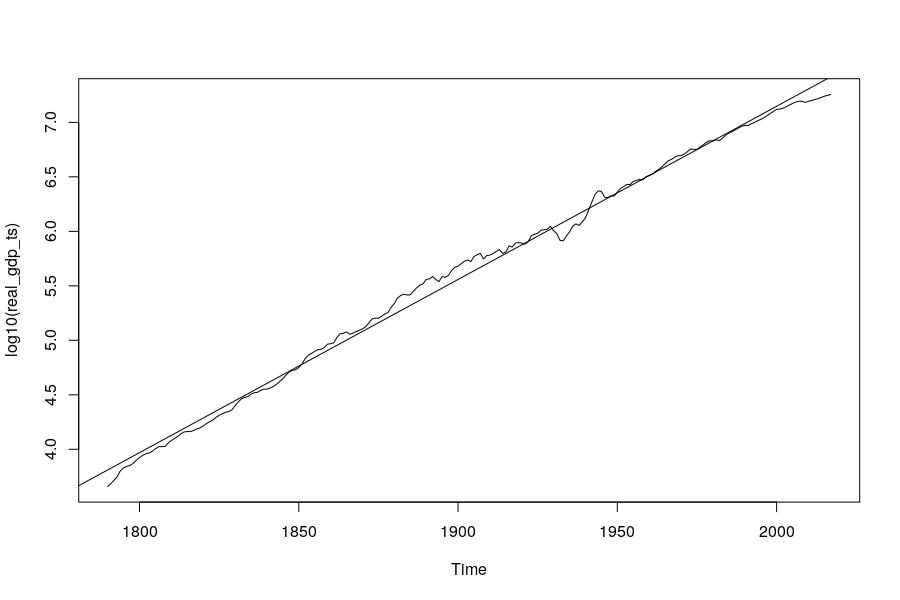
\includegraphics[width=0.49\linewidth]{PBI_log_tend.png}}
	\caption{PBI real (izquierda) y logaritmo en base 10 del PBI real (derecha)} 	
	\label{fig:PBI_orig}
\end{figure}

A pesar de lo enormemente explicativa que es la tendencia lineal sobre el logaritmo de la serie, hay zonas en las que el residuo es estrictamente positivo o negativo, por lo que puede analizarse si hay ciclos en estos residiuos, es decir, alrededor de la tendencia lineal. Los residuos pueden visualizarse en la figura \ref{fig:PBI_cntr}.

\begin{figure}[H]
	\centering
    \subfigure{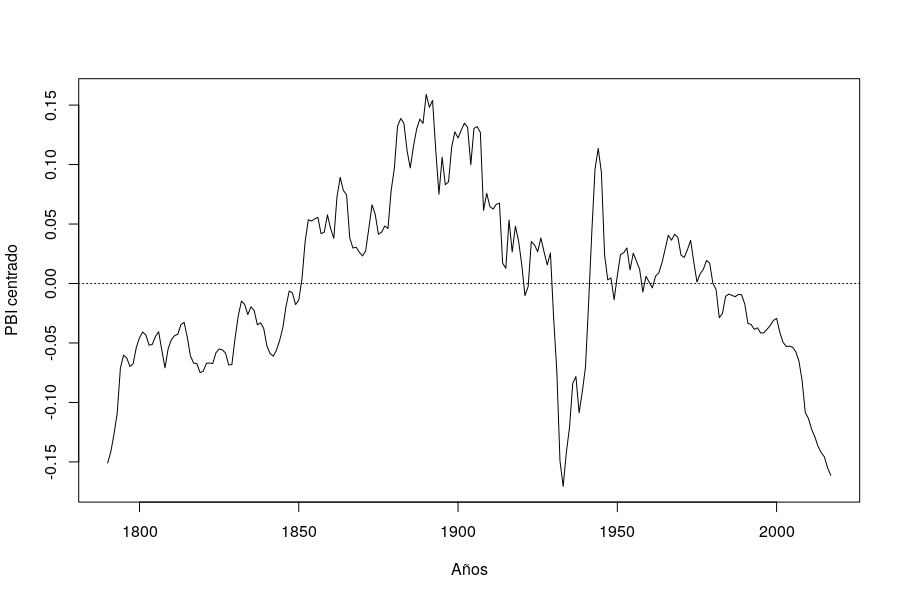
\includegraphics[width=0.8\linewidth]{PBI_centrado.png}}
	\caption{PBI centrado por la tendencia lineal} 	
	\label{fig:PBI_cntr}
\end{figure}


Nuevamente, aplicamos la transformada de Fourier sobre los residuos. Puede observarse el módulo de los vectores formados con respecto a la frecuencia en la figura \ref{fig:PBI_cntr_fft}.

\begin{figure}[H]
	\centering
    \subfigure{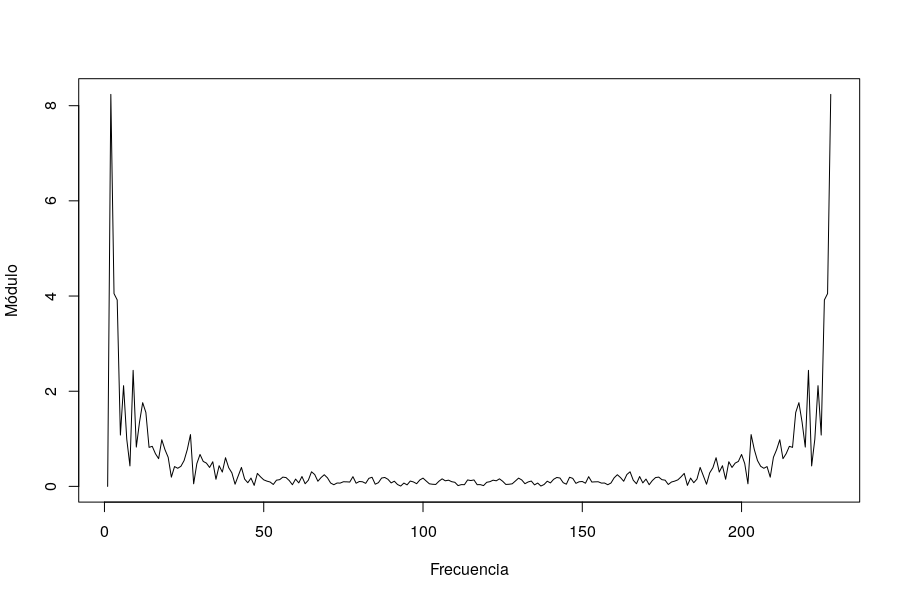
\includegraphics[width=0.8\linewidth]{PBI_centrado_fft.png}}
	\caption{Transformada de Fourier del PBI centrado} 	
	\label{fig:PBI_cntr_fft}
\end{figure}

Luego podemos observar el ajuste de la transformada de Fourier a los datos. Para ello graficamos nuevamente los residuos y la anti-transformada de las frecuencias más bajas de la transformada de Fourier expuesta previamente. Esto se puede observar en \ref{fig:PBI_cntr_antifft}

\begin{figure}[H]
	\centering
    \subfigure{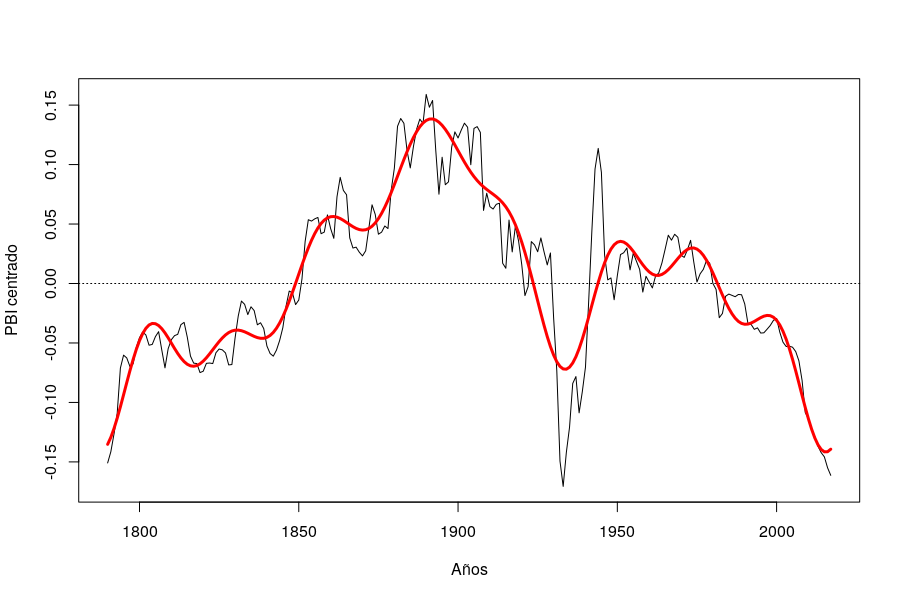
\includegraphics[width=0.8\linewidth]{PBI_centrado_antifft.png}}
	\caption{Serie original y antitransformada de las frecuencias más bajas} 
	\label{fig:PBI_cntr_antifft}
\end{figure}

Nuevamente observamos los residuos explicados de la serie y la autocorrelación de esos residuos en \ref{fig:PBI_fft_resid}. Puede observarse que aún queda estructura por explicar en los residuos dado por ciclos de más baja frecuencia. Esto demuestra que se puede descomponer la serie en ciclos de baja y alta frecuencia, si bien en este estudio estamos mayormente interesados en ciclos de largo plazo (señales de baja frecuencia y alta amplitud).

\begin{figure}[H]
	\centering
    \subfigure{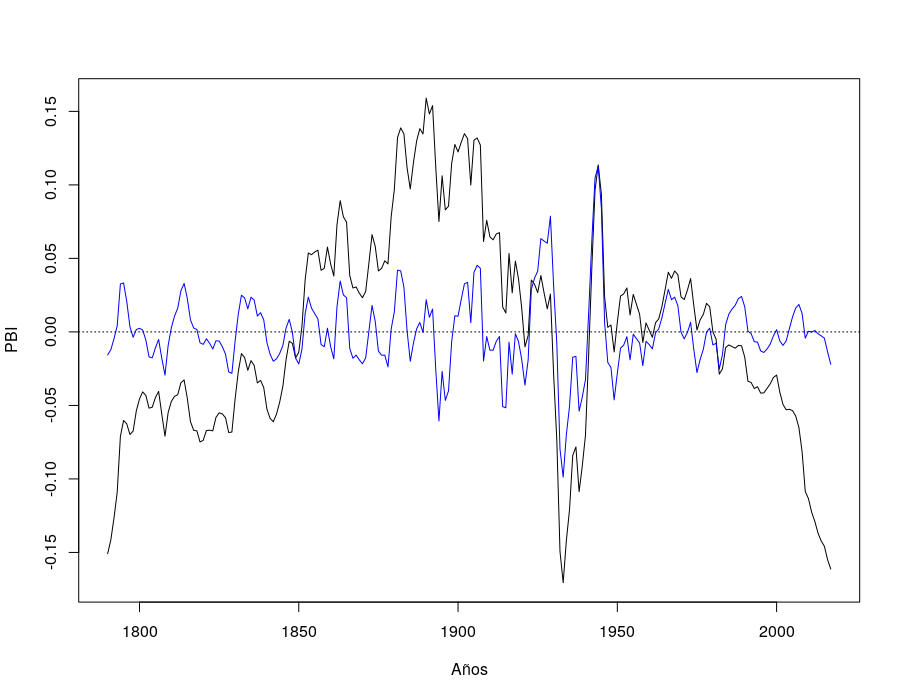
\includegraphics[width=0.49\linewidth]{PBI_fft_resid.png}}
	\subfigure{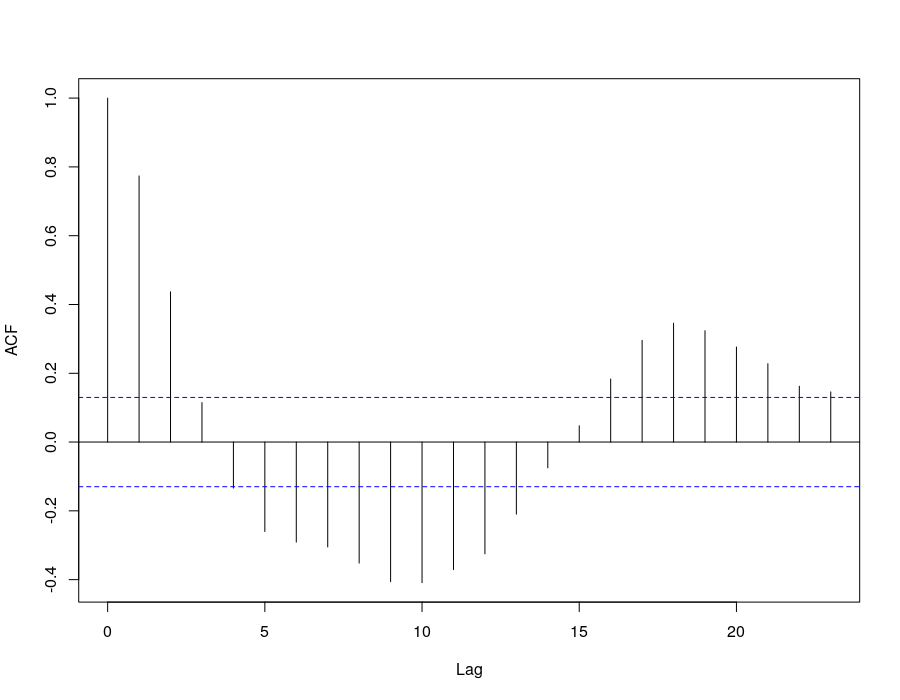
\includegraphics[width=0.49\linewidth]{PBI_resid_acf.png}}
	\caption{PBI centrado con residuos en azul (izquierda) y ACF de los residuos (derecha)}
	\label{fig:PBI_fft_resid}
\end{figure}

\end{document}
